\documentclass{beamer}
\usetheme{CambridgeUS}

\setbeamertemplate{caption}[numbered]{}

\usepackage{enumitem}
\usepackage{tfrupee}
\usepackage{amsmath}
\usepackage{amssymb}
\usepackage{gensymb}
\usepackage{graphicx}
\usepackage{txfonts}

\def\inputGnumericTable{}

\usepackage[latin1]{inputenc}                                 
\usepackage{color}                                            
\usepackage{array}                                            
\usepackage{longtable}                                        
\usepackage{calc}                                             
\usepackage{multirow}                                         
\usepackage{hhline}                                           
\usepackage{ifthen}
\usepackage{caption} 
\captionsetup[table]{skip=3pt}  
\providecommand{\pr}[1]{\ensuremath{\Pr\left(#1\right)}}
\providecommand{\cbrak}[1]{\ensuremath{\left\{#1\right\}}}
\renewcommand{\thefigure}{\arabic{table}}
\renewcommand{\thetable}{\arabic{table}}                                     
                               
\title{AI1110 \\ Assignment 8}
\author{U.S.M.M TEJA \\ CS21BTECH11059}
\date{17th May 2022}


\begin{document}
	% The title page
	\begin{frame}
		\titlepage
	\end{frame}
	
	% The table of contents
	\begin{frame}{Outline}
    		\tableofcontents
	\end{frame}
	
	% The question
	\section{Question}
	\begin{frame}{question 4.13}
A fair coin is tossed three times and the random variable x equals the total number of heads.
Find and sketch $F_x(x)$ and $f_x(x)$.
	\end{frame}
	
	% The solution
	\section{Solution}
	\begin{frame}{Events}
let x be a random variable which maps to 1 when coin denotes head and 0 when it denotes tail.

\begin{table}[ht!]
		\centering
		\input{tables/table-1.tex}
		\caption{Events and Description}
		\label{table:1}
\end{table}
    \end{frame}

\begin{frame}{calculations}
 \begin{align}
     &\pr{X=0} = \binom{3}{0}\times \frac{1}{2}^0 \times (1-\frac{1}{2})^3 = \frac{1}{8}& \\
 &\pr{X=1} = \binom{3}{1}\times \frac{1}{2}^1 \times (1-\frac{1}{2})^2 = \frac{3}{8}& \\   
 &\pr{X=2} = \binom{3}{2}\times \frac{1}{2}^2 \times (1-\frac{1}{2})^1 = \frac{3}{8}& \\
 &\pr{X=3} = \binom{3}{3}\times \frac{1}{2}^3 \times (1-\frac{1}{2})^0 = \frac{1}{8}& 
\end{align}   
\end{frame}

\begin{frame}{PMF}
 the $F_x(x)$ i.e PMF is given by :
 \begin{equation}
 \begin{cases}
 0, & k < 0 \\
 \frac{1}{8}, & k = 0 or 3 \\
 \frac{3}{8}, & k = 1 or 2
 \end{cases}
 \label{cdf}
 \end{equation}
\end{frame}

\begin{frame}{CDF}
    the $f_x(x)$ CDF is given by :
 \begin{equation}
 \begin{cases}
 0, & k < 0 \\
 \frac{1}{8}, & k = 1 \\
 \frac{1}{2}, & k = 2 \\
 \frac{7}{8}, & k = 3 \\
 1, & k> 3 \\ 
 \end{cases}
 \label{cdf}
 \end{equation}
\end{frame}

\begin{frame}{plots for PMF and CDF}
  \begin{figure}[!ht]
\centering
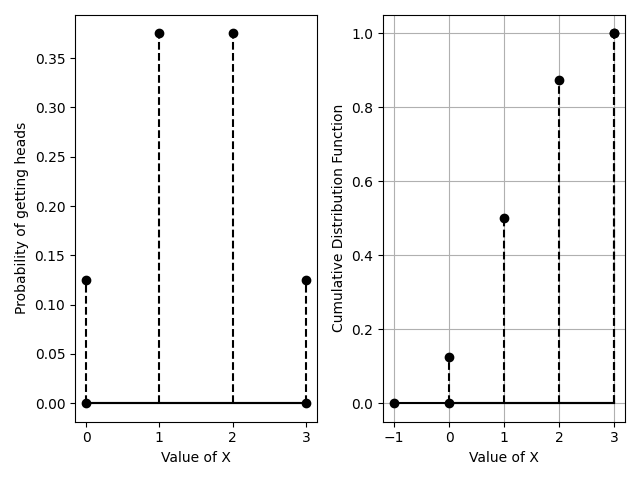
\includegraphics[width=\columnwidth]{9.png}
\caption{Plot of the PMF (left) and CDF (right) of an unbiased die.}
\label{fig:pmf-cdf}
\end{figure}
   
\end{frame}
\end{document}
